\section{GM-7. Strategy}

\subsection*{Problema}
El movimiento depende del dispositivo de entrada, pero el personaje debe conservar las mismas reglas de límites, velocidad y efectos.

\subsection*{Contexto}
Se permite teclado o ratón/táctil; versus asigna teclas distintas a cada jugador.

\subsection*{Solución y aplicación}
\texttt{Personaje} es el contexto; \texttt{ControlMovimiento} es la estrategia; \texttt{ControlTeclado} y \texttt{ControlTactil} son las implementaciones. Se inyecta el control al construir la partida y el personaje delega en él en cada actualización. El teclado calcula una dirección y el táctil convierte coordenadas mediante \texttt{Viewport.unproject()}.

\subsection*{Evidencia}
\begin{itemize}
\item \href{https://github.com/maverick1006/Proyecto-Game-LLuvia-/blob/entrega-final/core/src/main/java/puppy/code/ControlMovimiento.java#L4}{ControlMovimiento.java, línea 4} (\texttt{void actualizar(})
\item \href{https://github.com/maverick1006/Proyecto-Game-LLuvia-/blob/entrega-final/core/src/main/java/puppy/code/Personaje.java#L41}{Personaje.java, línea 41} (\texttt{control.actualizar(this, delta)})
\item \href{https://github.com/maverick1006/Proyecto-Game-LLuvia-/blob/entrega-final/core/src/main/java/puppy/code/ControlTeclado.java#L11}{ControlTeclado.java, línea 11} (\texttt{public void actualizar(})
\item \href{https://github.com/maverick1006/Proyecto-Game-LLuvia-/blob/entrega-final/core/src/main/java/puppy/code/ControlTactil.java#L16}{ControlTactil.java, línea 16} (\texttt{viewport.unproject})
\item \href{https://github.com/maverick1006/Proyecto-Game-LLuvia-/blob/entrega-final/core/src/main/java/puppy/code/GameLluvia.java#L50}{GameLluvia.java, línea 50} (\texttt{private void iniciar()})
\end{itemize}

\clearpage
\begin{figure}[p]
\centering
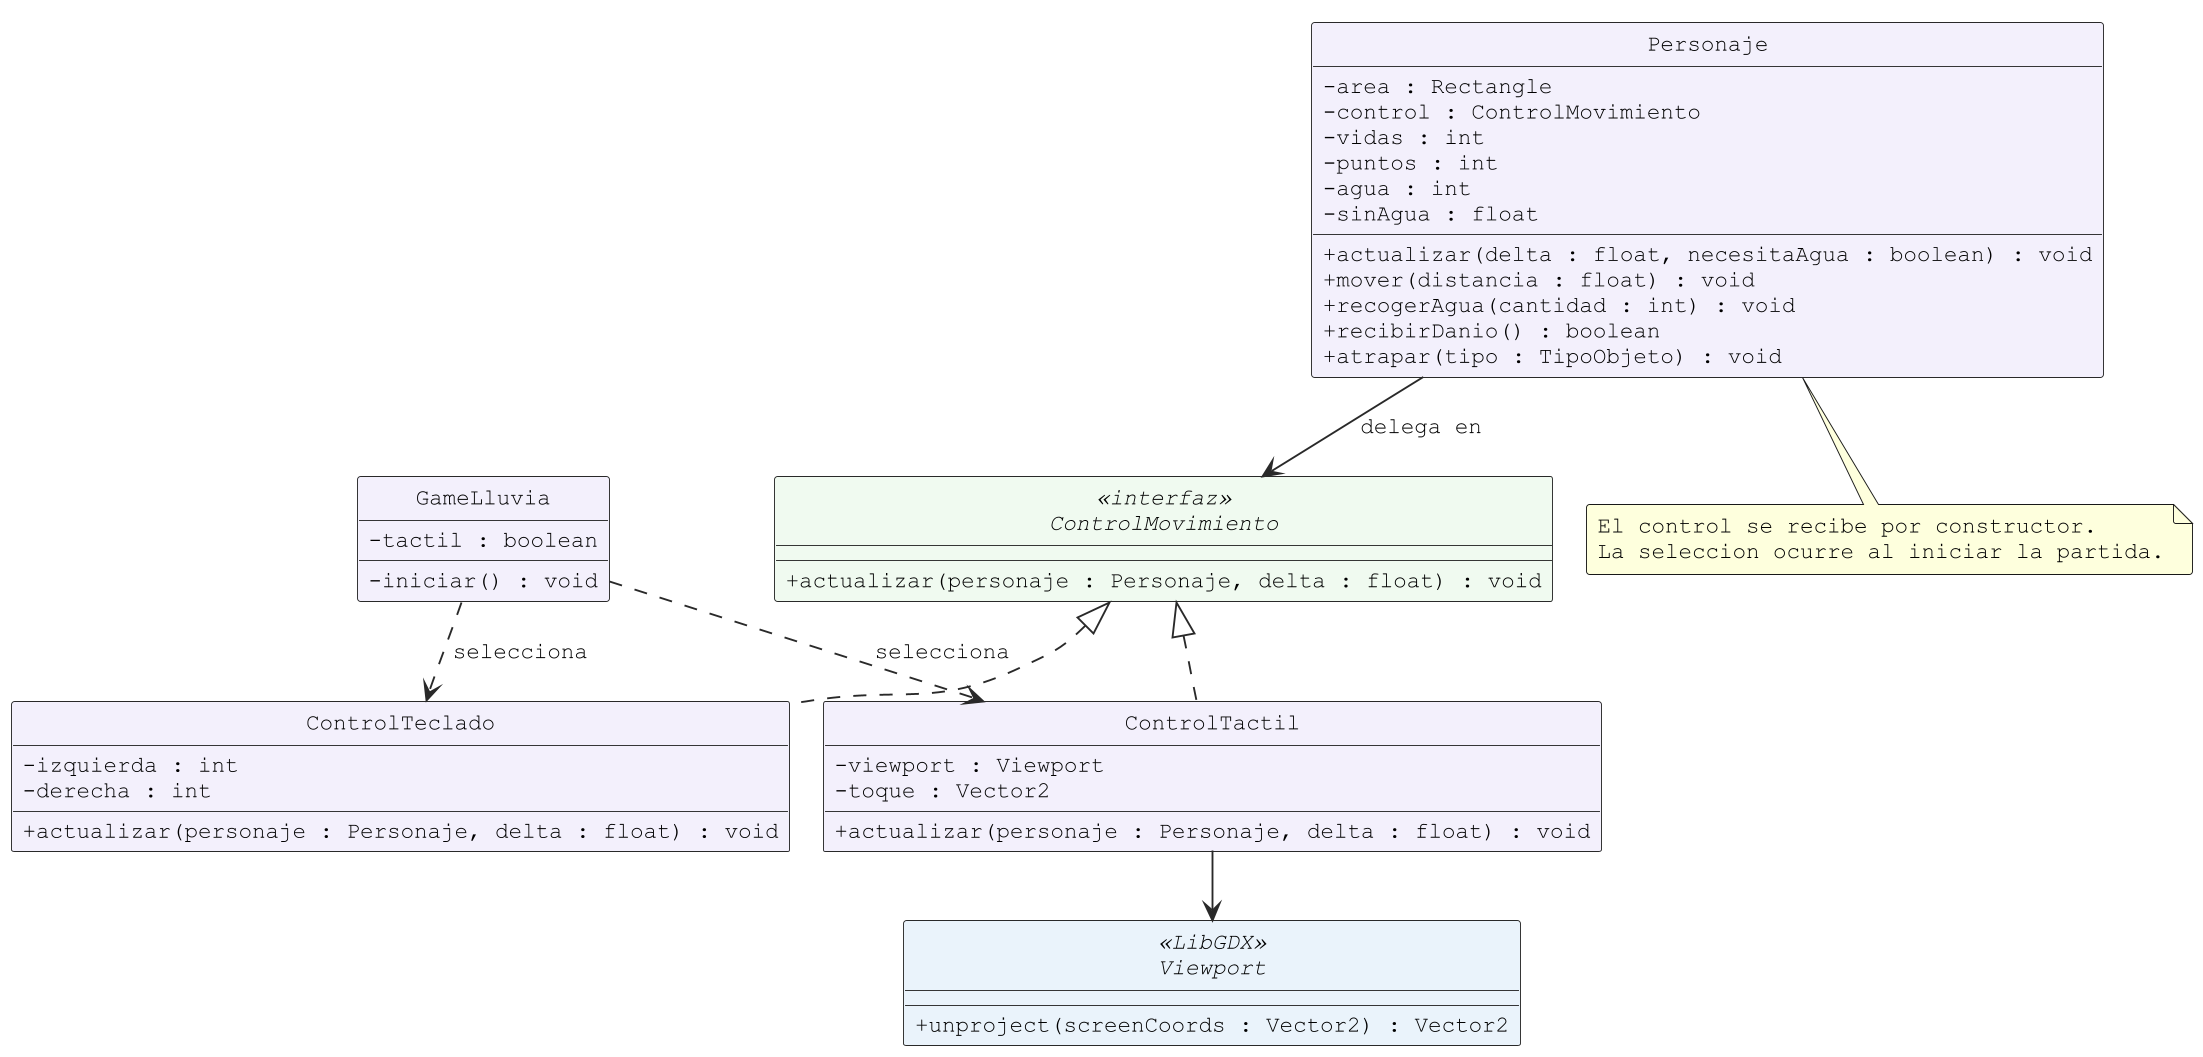
\includegraphics[width=0.95\linewidth,height=0.84\textheight,keepaspectratio]{images/03-strategy.png}
\caption{Strategy aplicado al movimiento del personaje}
\end{figure}




